
% ----------------------------------------------------------
\begin{frame}
  \frametitle{Circuit Optimation for Application}
  Optimization takes advantage of allowed transformations (e.g. commutation
  and cancellation) to reduce gate count, decrease circuit depth,
  accommodate gate set, etc. 
  \begin{columns}
    \column[T]{0.65\linewidth}
    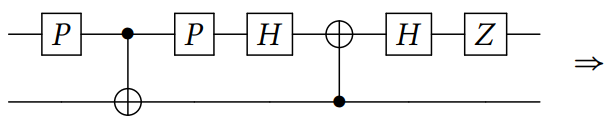
\includegraphics[width=\linewidth]{Graphics/Q-cancellation-optimizer.png}

    \column[T]{0.35\linewidth}  
    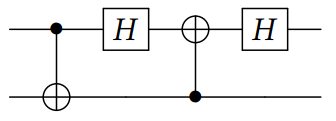
\includegraphics[width=\linewidth]{Graphics/Q-cancellation-optimized.png}
  \end{columns}
  \begin{center}
    \vspace*{-\baselineskip}
    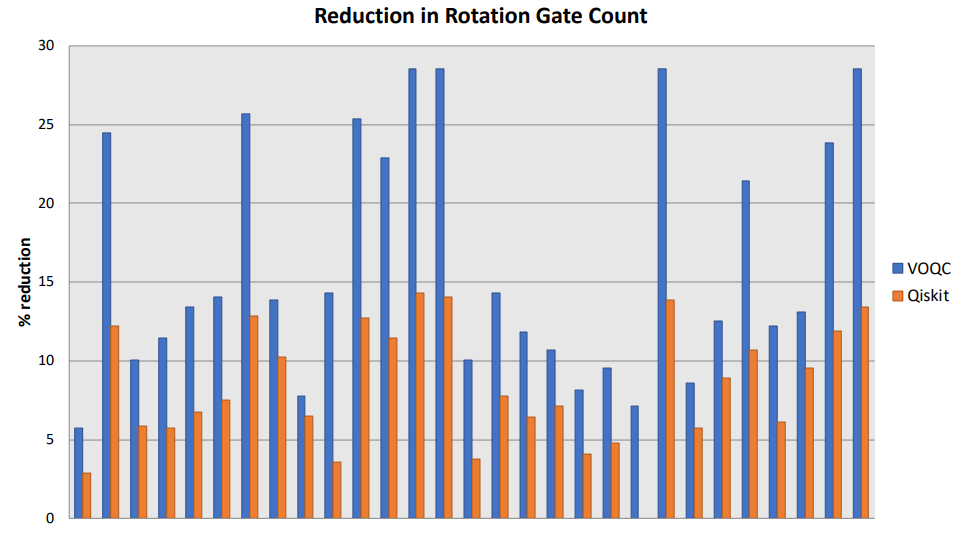
\includegraphics[width=0.55\linewidth]{Graphics/Rotation-gate-reduction-VOQC.png}
  \end{center}

  Verified Optimizer for Quantum Computing (VOQC)~\cite{VOQC}
\end{frame}
